\documentclass [11pt,fleqn]{article}

\usepackage{amssymb}
%\usepackage{epsf,psfig,graphicx}
%\usepackage{epstopdf} % TJL ADDED
\usepackage{bm}
\usepackage{epsf,graphicx}
\usepackage{psfrag}
\usepackage{amsmath}
\usepackage{color}
\topmargin     -0.60in  % (adjusted for printer bias) 
\headheight      .00in  % (no headers) 
\headsep         .50in  % (top margin + headers + skip) 
\textheight     9.50in  % (instructions: 9 1/8'' min, 9 7/16'' max) 
\textwidth      6.00in  % 2*3.33 + .33 = 6.99 
\oddsidemargin  0.3125in  % (subtracted 1inch bias) 
\evensidemargin 0.3125in 
%\renewcommand{\baselinestretch}{1.5} 
\parindent .0in 
\parskip 10pt 


\font \bigtenrm=cmmi10 scaled\magstep2 
\def \dt {\delta\tau} 
\def \ve {\varepsilon} 
\def \ch {{\cal H}} 
\def \del {\partial} 
\def \be {\begin{equation}} 
\def \ee {\end{equation}} 
\def \beq {\begin{eqnarray}} 
\def \eeq {\end{eqnarray}} 
\def \tv {\tilde v} 
\def \veren {\varepsilon^{\rm ren}_f} 
\def \vef {\varepsilon^0_f} 
\def \su {\uparrow} 
\def \sd {\downarrow} 
\def \CR {\nonumber\\} 
\def \hfb {\hfill\break} 
\def \tb {\bar{t} } 
\def \kb {\bar{k} } 
\def \tbB {\bar{t}_B } 
\renewcommand*{\thefootnote}{\fnsymbol{footnote}}
%\def \ul{#1} {$\underline{#1 }$}

\usepackage{authblk}

\title{Observation of correlated x-ray scattering at atomic resolution}
\author[1]{ Derek Mendez }
\author[3]{ Thomas J. Lane}
\author[1,2]{Jongmin Sung}
\author[6]{Jonas Sellberg}
\author[4]{Cl\'ement Levard}
\author[1]{Herschel Watkins}
\author[6]{Aina E. Cohen}
\author[6]{Michael Soltis}
\author[2,5]{Shirley Sutton}
\author[2]{James Spudich}
\author[3]{Vijay Pande}
\author[6]{Daniel Ratner}
\author[1,6]{Sebastian Doniach\thanks{corresponding author: sxdwc@slac.stanford.edu}}

\affil[1]{Stanford University Department of Applied Physics, Stanford, CA 94305}
\affil[2]{Stanford University Department of Biochemistry, Stanford, CA 94305}
\affil[3]{Stanford University Department of Chemistry, Stanford, CA 94305}
\affil[4]{Aix-Marseille Universit\'e, CNRS, IRD, CEREGE UM34, 13545 Aix en Provence, France}
\affil[5]{Stanford University School of Medicine, Stanford, CA 94305}
\affil[6]{SLAC National Accelerator Laboratory, Menlo Park, CA 94025}

\renewcommand\Authands{ and }
\date{}
\begin{document} 

\maketitle

{\bf Abstract}

Tools to study disordered systems with local structural order, such as proteins in solution, remain limited. Such understanding is essential for \emph{e.g.}~rational drug design. Correlated x-ray scattering (CXS) has recently attracted new interest as a way to leverage next-generation light sources to study such disordered matter. The CXS experiment measures angular correlations of the intensity caused by the scattering of x-rays from an ensemble of identical particles, with disordered orientation and position. Averaging over 15,496 snapshot images obtained by exposing a sample of silver nanoparticles in solution to a micro-focused synchrotron radiation beam, we report on experimental efforts to obtain CXS signal from an ensemble in three dimensions. A correlation function was measured at  wide angles corresponding to atomic resolution that matches theoretical predictions. These preliminary results suggest that other CXS experiments on disordered ensembles -- such as proteins in solution -- may be feasible in the future.


{\bf Keywords/phrases} 

x-ray angular correlations, silver nanoparticles, atomic resolution x-ray scattering, synchrotron radiation, solution ensemble, double Bragg scattering

\section{Introduction}

In a pioneering paper, Kam \cite{Kam:1977wc} showed that correlated x-ray scattering (CXS) from an ensemble of randomly oriented particles could in principle reveal information about the internal structure of the particles beyond usual small and wide angle solution scattering measurements. The extraction of such information in the absence of an ordered system (\textit{e.g.}~a crystal) can be beneficial in biological studies, as many biological systems with well defined local structural order are inherently disordered at large length scales.

In order to gauge the feasibility of Kam's method at atomic resolution and to assess the associated difficulties, we conducted experiments measuring CXS from silver nanoparticle (NP) solutions at wide angles. Crucially, each measurement was conducted on an ensemble of NPs oriented randomly in three dimensions, extending previous experimental work done in two dimensions \cite{Saldin:2011ch}, at small angles \cite{Kam:1981ua, Wochner:2009ia}, or on single particles \cite{Kam:1985tz, Starodub:1fy}. 

From these experiments, we obtained empirical correlation functions between all pixel pairs in two silver Bragg rings, corresponding to Miller indices 111 and 200. Preliminary analysis of the three correlation functions (two rings correlated with themselves and with each other) show sharp peaks consistent with analytical and simulated predictions based on the crystal structure of silver.

By successfully measuring CXS signal from randomly oriented ensembles of silver NPs, we have demonstrated the effectiveness of Kam's method at atomic resolution. This experiment will serve as a benchmark for future experiments involving weaker scatterers, such as proteins. Refinement of our experimental technique on a well characterized sample (\textit{i.e.}~silver NPs) will also help facilitate the extension of CXS to studies of biomolecules in solution.

\section{Theory}

\begin{figure}
\begin{center}
\includegraphics[ ]{./setup.eps}
\end{center}
\caption{Experimental setup: a kapton capillary filled with a solution of silver NPs (face-centered-cubic). Bragg rings $q_{111}$ and $q_{200}$ are illustrated by circles on the detector plane. At least one of the exposed NPs happens to be oriented such that two reciprocal lattice (body-centered-cubic) peaks are intersecting the detector at $q_{111}$. Dashed lines represent the scattering vectors (separated by the angle $\psi$), and solid lines represent the projection of those vectors onto the detector plane (separated by the angle $\Delta$). Artwork courtesy of Gregory M.~Stewart (SLAC).}
\label{fig:setup}
\end{figure}

We briefly review the portions of \cite{Kam:1977wc} relevant to this paper. Let $S( \bm q,\omega)$ represent the structure factor of an isolated particle in solution, \textit{i.e.}
\be \label{structurefactor}
S(\bm q,\omega) = \left| \> \sum_{j}^{N_j} f_j (q )e^{i \bm q \cdot  \left( \hat{R}_\omega \cdot \bm r_j\right)  } \right| ^{2}
\ee
where $\bm q$ is the scattering momentum transfer vector,  $\bm r_j$ and $f_j (q )$ are the coordinates and form factor of the $j^{th}$ atom in the particle respectively $( 1 \leq j \leq N_{j} )$, $\omega$ is a triple of Euler angles, $\hat{R}_\omega$ is a three-dimensional rotation operator, and the sum is over all $N_j$ atoms in the particle.

Kam showed that if the distribution of particle rotations dictated by $\hat{R}_\omega$ is isotropic, distributed uniformly over $\omega$, then the scattering factor correlation function
\be \label{correlation}
C(\bm q_1, \bm q_2) = \frac{N}{8 \pi^{2}}\int S( \bm q_{1},\omega ) S( \bm q_{2},\omega ) \, d \omega
\ee
may be extracted from a CXS measurement where one repeatedly records snapshots of a $N$-particle solution, with each snapshot representing a unique ensemble of the particles frozen in three-dimensional space. Kam showed (assuming negligible inter-particle scattering interference) that the empirical correlation function averaged over shots would converge to (\ref{correlation}), \textit{i.e.},
\be \label{converge}
\big \langle   n_s(\bm q_1)  \, n_s(\bm q_2) \big \rangle_s  - \big \langle {n}_s(\bm q_1) \big \rangle_s \, \big \langle {n}_s(\bm q_2) \big \rangle_s   \Rightarrow C(\bm q_1, \bm q_2) 
\ee
where $n_{s}(\bm q)$ is the total photons scattered from all particles in snapshot $s$ into a pixel along scattering vector $\bm q$. Neglecting inter-particle scattering interference, $n_{s}(\bm q)$ can be thought of as a probabilistic linear combination of $S(\bm q,\omega)$ for a set of orientations $\{ \omega\}_{s}$.

In the special case of an isotropically oriented sample, Kam proved that the absolute orientation of the $\bm q_1, \bm q_2$ scattering pair in the correlation function is irrelevant; the relevant covariates are only the magnitudes $| \bm q_1 | , | \bm q_2 | $ and the angle between the vectors, $\psi$. Thus the correlation function can be written 
\[
C(\bm q_1, \bm q_2)  \equiv C (q_1,q_2, \psi  )
\]
Experimentally, we statistically estimate this function by taking angular correlations in the detector plane; let $\phi$ be the azimuthal coordinate of $\bm q$ projected into the plane perpendicular to an incident beam (corresponding to the azimuthal coordinate of a pixel measuring $\bm q$ on a farfield planar detector). Let $\Delta = |\phi_{1} - \phi_{2}|$ be the angle between two such vector projections. Then define the average angular correlation of ring intensity fluctuations as
\be \label{angular}
D (q_1,q_2, \Delta  ) = \left \langle \int_{0}^{2\pi}  \Big ( n_s(q_1,\phi) -   \mu_s( q_1) \Big) \Big ( n_s(q_2,\phi + \Delta) -   \mu_s( q_2) \Big)  \, d\phi  \right \rangle_{s}
\ee

where $\mu_s( q)$ is the average photon counts at $q$ in snapshot $s$. Assuming randomly oriented particles, negligible inter-particle scattering (wide angles and/or a dilute sample), and a sufficiently large number of snapshots, $D (q_1,q_2, \Delta)$ will converge to a statistical estimate of the Kam correlation $C (q_1,q_2, \psi)$, up to a trigonometric conversion of $\Delta$ (the angle between $\bm q_1, \bm q_2$ projections on the plane of the detector) and $\psi$ (the angle between $\bm q_1, \bm q_2$).

We have computed the expected angular correlation function (\ref{angular}) for the silver NPs studied as a benchmark for our experimental results (Figure \ref{fig:results}-B). A silver NP may be represented by a simple model consisting of a face-centered-cubic lattice cutoff by a spherical boundary. The scattering can then be represented by reciprocal lattice vectors cutting the Ewald sphere and giving rise to Bragg peaks. Hence, each snapshot records a series of Bragg rings (henceforth we will only consider scattering vectors which meet the Bragg condition for silver, denoted by a set of Miller indices, $\bm q_{hkl}$). The sub-population of all NP orientations that simultaneously subtend two Bragg peaks on the Ewald sphere give rise to angular correlations. Therefore,  CXS signal appears at values of $\Delta $ corresponding to the geometry of the reciprocal lattice and the angles between reciprocal lattice vectors (Figure \ref{fig:setup}). For instance, we calculate that $D (q_{111},q_{111}, \Delta  )$ should display strong signal at $\Delta_1 = \arccos[ \frac{-2}{3\cos^{2}\theta} + 1  ]$ and $\Delta_2 = \arccos[ \frac{-4}{3\cos^{2}\theta} + 1  ]$ where $2\theta$ is the standard scattering angle.


It is clear that the function $C(\bm q_1, \bm q_2)$ in (\ref{correlation}) contains information about the structure of the particles under study. Even though one can show that inverting a complete set of such correlations to an image of the electron density (at arbitrary resolution) is an underdetermined problem \cite{Elser:2011ez}, we would like to emphasize that (\ref{correlation}) can be calculated using a model for the structure factor (\ref{structurefactor}) defined by a particle's atomic positions. This opens up the possibility for refining such a model against a CXS dataset using (\ref{converge}) \cite{Liu:2013dv, Chen:2013io, Saldin:2009jj}, especially in cases where prior information (such as protein primary sequence) can be included. Other routes to analyzing structure given CXS data include iterative phasing \cite{Saldin:2010bx}, implicit alignment of particles \cite{Poon:2013ia}, or direct analysis of local internal symmetries of the system \cite{Kurta:2012cb, Kurta:2013to}.


Theoretical results suggest the CXS signal to noise scales as $\sqrt{N_{s}}$ , but is independent of the number of illuminated particles $N $, for large $N$ \cite{Kam:1977wc, Kam:1981ua, Kirian:2011bq}. These facts were employed to optimize our experimental design, which emphasized collecting a large number of independent snapshots.

\section{Methods}

\begin{figure}
\begin{center}
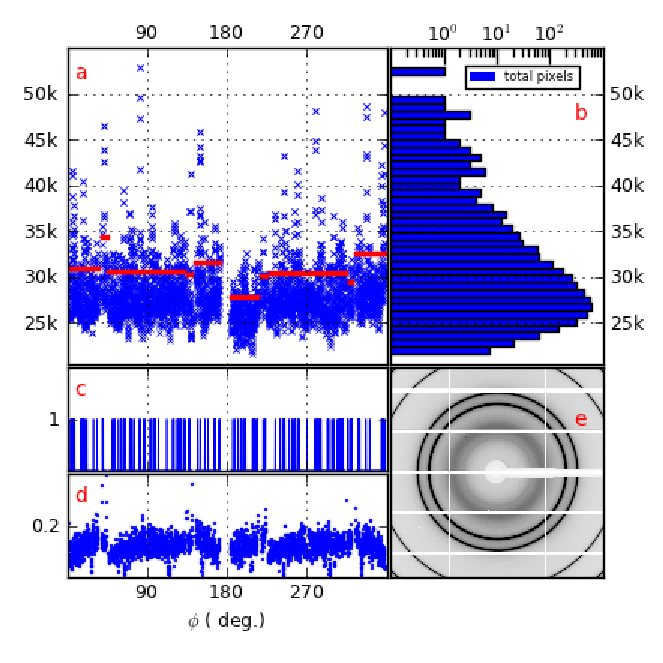
\includegraphics[ ]{./binary.eps}
\end{center}
\caption { {\bf a)} Representative measurement of one x-ray snapshot, $n_{s}( q_{111},\phi)$, \textit{i.e.}~the photon counts around the Bragg ring at $q_{111}$. The horizontal bars show the binary cutoff along the ring for each module. Here, the $q_{111}$ ring spans 10 modules in total. {\bf b)} Histogram of the intensities in {\bf a} on a log scale of photon numbers. Notice the tail at higher intensities, indicating the presence of large particles. {\bf c)} Result of applying the binary filter to {\bf a}. On average, a binary shot at $q_{111}$ is 10\% ones, 77\% zeros and 13\% masked pixels (masked pixels are ignored in the analysis).  {\bf d)} The average binary intensity from a scan of 500 snapshots. Notice systematic structure in the intensity response, indicating intra-module pixel variations. {\bf e)} Typical snapshot showing the Bragg rings at $q_{111}$ and $q_{200}$. Low/high intensities shown in white/black.}
\label{fig:binary}
\end{figure}


Data from 15,496 x-ray diffraction images \cite{data} of silver NP solution were collected and analyzed at the micro-focus crystallography beamline (12-2) at SSRL. We prepared a sample containing an estimated $10^{9}$  20 nm NPs per snapshot in the illuminated volume, but we observed significant numbers of NPs that were larger. Samples were loaded and oriented in the X-ray beam using the Stanford Automated Mounting System (SAM) \cite{Cohen:2002jw}, controllable from the experimental hutch. Using a liquid nitrogen-cooled double crystal monochromator we tuned the beam energy to 17 keV. The beam was focused down to about $20 \times 50 \,\mu$m$^2$ using Rh coated Kirkpatrick-Baez mirrors and had a flux of $2\times 10^{12}$ photons per second. Snapshots were recorded on a Dectris Pilatus 6M photon counting detector. 

To successfully measure a correlation function via the scheme (\ref{converge}), the sample must be frozen in time or space. Any random motion due to diffusion of particles will reduce the scattering correlation, which is a function of the particle structure and orientation (\ref{structurefactor}). To prevent diffusion during the long exposure times (order 1 second) necessary to scatter a sufficient number of photons to measure a correlation signal at a synchrotron, we cooled the sample using an Oxford Instruments Cryojet, ensuring that the particles remained immobilized during each exposure. Further, no changes in the diffraction images were observed during the course of a single snapshot exposure, indicating the sample did not undergo significant diffusion or radiation damage.

The silver NPs, coated in PVP, were synthesized following a protocol described elsewhere \cite{Levard:2011bx}. In order to prevent the formation of solvent crystals at the low temperature, the NPs were concentrated and suspended in 80\% glycerol and 3\% agarose with a final concentration of 350 mg/ml. The solutions were held in kapton capillaries (500 and 600 $\mu$m inner and outer diameter, respectively) and flash frozen in liquid nitrogen. Kapton and glycerol scatter into relatively lower angles, and did not corrupt our silver NP signal.

Our goal was to record as many snapshots as possible, each one representing a different ensemble of particle orientations frozen in time. The sample holder was equipped to automatically rotate the capillary 150 degrees about its longitudinal axis, perpendicular to the beam. Photon counts were read out and reset every 0.7 second as the capillary rotated 0.3 degrees under continuous beam irradiation, yielding 500 shots per 150 degree rotational scan. This was deemed an optimal timing to simultaneously maximize signal and minimize damage and heating. Every 500 shots, between scans, the capillary was moved longitudinally so as to always probe different regions of the sample.

A bicubic interpolation algorithm was used to convert the cartesian pixel lattice to polar coordinates for calculation of (\ref{angular}). Using the Scherrer equation [8] relating the width of a Bragg ring to the average NP size, we concluded that the majority of silver NPs in each snapshot were roughly 20 nm in diameter. Histograms of photon counts into the $q_{111}$ Bragg ring indicate a rather large distribution of particle sizes (Figure \ref{fig:binary}-B) which we discuss in the following section.

\section{Results}


\begin{figure}
\begin{center}
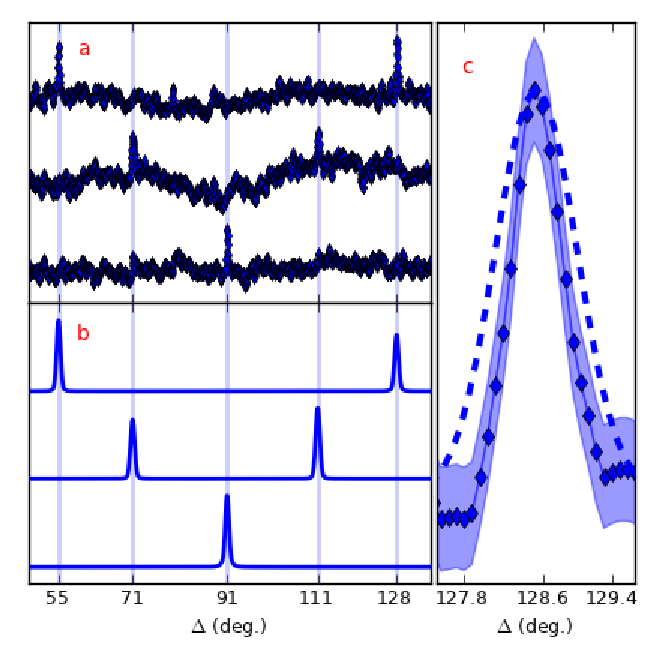
\includegraphics[ ]{./results.eps}
\end{center}
\caption{ {\bf a)} From top to bottom, measured correlation functions $D (q_{111},q_{200}, \Delta  )$, $D (q_{111},q_{111}, \Delta  )$, and $D (q_{200},q_{200}, \Delta  )$ from 20 nm silver nanoparticles. {\bf b)} Corresponding simulations of the correlations plotted in {\bf a}. Vertical lines mark analytical predictions. We truncated the angular range to highlight the correlation peaks. Regions not shown contain artifacts similar to those on the figure, with nothing greater in magnitude than the CXS peaks. {\bf c)} Simulation (dashed line) and measurement (diamond marker) of a correlation peak width. The simulation was for 20 nm particles. Peak width scales inversely with particle size, hence we expect the measured CXS resulted from particles larger than 20 nm. Shading represents 95\% confidence intervals on the measurement. }
\label{fig:results}
\end{figure}

Here we report on our attempts to resolve (\ref{angular}) at the two brightest silver Bragg rings. Specifically, we calculated $D (q_{111},q_{200}, \Delta  )$, $D (q_{111},q_{111}, \Delta  )$, and $D (q_{200},q_{200}, \Delta  )$. 

Convergence of the CXS signal is complicated by the inherent statistical noises described in [1,7], and CXS measurement is sensitive to systematic noises associated with the experimental conditions \cite{Kam:1981ua}, \textit{e.g.}~detector artifacts. The Pilatus 6M detector is made up of 60 pixel modules separated by 1-2 mm gaps, and each Bragg ring subtends multiple modules. The overall electronic response of each module is slightly different, causing systemic anisotropies which lead to detector intensity correlations that dominate the sample CXS. 

Unprocessed estimates of the correlation function (\ref{angular}) in the data we obtained are dominated by such systematic artifacts. To mitigate these effects, we apply a binary filter to the data (Figure \ref{fig:binary}). We define the filter as follows: Let $\{ \bm q_{hkl} \}_{m}$ represent the set of Bragg pixels on the $m^{th}$ detector module ($1 \leq m \leq 60$). Let $\mu_m$ and $\sigma_m$ represent the average and standard deviation of $n_{s}(\bm q)$  for all $\bm q \in \{ \bm q_{hkl} \}_{m} $, respectively. Then for each $\bm q \in \{ \bm q_{hkl} \}_{m} $, we apply the photon count filter:

\[  n_{s}(\bm q ) = 
 \begin{cases} 
   1 & \quad \text{if } n_{s}(\bm q ) > \mu_m +  \sigma_m\\
   0 & \quad \text{otherwise} 
 \end{cases} 
 \]

\textit{i.e.}~per module, all Bragg pixels less than one standard deviation above the mean are set to zero and the rest are set to unity. The threshold $\mu_m + \sigma_m$ was sufficient for our purposes and was not optimized. The binary filter is a simple method for emphasizing the local variations from the sample compared to the background fluctuations of the detector; placing each detector module on the same scale removes correlations between modules.  After applying the filter and calculating (\ref{angular}), the resulting correlations reveal peaks that match the simulations and analytical predictions (Figure \ref{fig:results}). Despite the filtering, variations remain within each module which bias the binary filter selection and lead to the low frequency background correlations seen in Figure \ref{fig:results}-A. The binary filter is an intermediate stage in our on-going analysis; it provides a stepping stone to better data refinement techniques and CXS extraction.

As mentioned in the Methods section, we infer from the width of the Bragg rings that the majority of our sample consists of 20 nm silver NPs ($\sim10^9$ per snapshot). From tabulated coherent atomic cross sections \cite{Henke:1993wx} we estimate that each 20 nm silver NP scatters roughly 1.6 photons per 0.7 sec exposure. We can further estimate that roughly 8.3\% of these NPs scatter into the Bragg ring at $q_{111}$ on the detector. This is done by computing the volume each reciprocal lattice point occupies as the particle undergoes a complete set of rotations and then determining which fraction of that volume intersects the Ewald sphere. The reciprocal lattice site diameters were computed using the Scherrer equation [8]. These estimates are consistent with the average photon counts per pixel per snapshot in the $q_{111}$ Bragg ring, $\sim 4 \times 10^4$. 

However, many of the snapshots contained pixels at $q_{111}$ reporting photon counts as high as $\sim 8 \times 10^4$, much greater than one would expect given Poisson statistics, where fluctuations are order square-root of the mean. We therefore suspect our sample included a broad distribution of particle sizes, with larger particles scattering more photons. To gauge the approximate size of these particles we again employed the Scherrer equation, to relate the width of the correlation peak to the particle size (Figure \ref{fig:results}-C). The width of the measured correlation peak is consistent with 50 nm particles, thus we conclude that the measured correlations are most likely generated by scattering off of thousands of $\ge$ 50 nm particles per shot. We emphasize that this is an estimated lower bound on particle size; effects not included in the Scherrer equation (\textit{e.g.}~Brownian motion) can cause broadening of a Bragg peak. Of all 50 nm silver NP orientations, we estimate that roughly 0.19\% will simultaneously subtend two Bragg peaks on the detector into $q_{111}$, 0.06\% will simultaneously subtend two Bragg peaks on the detector into $q_{200}$, and 0.15\% will simultaneously subtend one Bragg peak into each of $q_{111}$, $q_{200}$.

We note that convergence of the correlations was not limited by the large number of randomly oriented particles in the beam.  At present, the main impediment to accurate measurements of CXS arises from anisotropy artifacts induced by the detector system.  We have been able to partially overcome background correlations by nonlinear binary filtering and are continuing data processing with more sophisticated methods.

\section{Conclusion}

Kam's original results \cite{Kam:1977wc} show that (\ref{correlation}), which may be directly calculated from the structure factors of the particle (\ref{structurefactor}), can be derived from measurement of an ensemble of particles. Hence accurate measurement of CXS in the three-dimensional $\{q_1,q_2,\Delta\}$ space can lead to constraints on a sample's electron density model, providing a route to iterative refinement of the sample structure (as in \cite{Schroder:2010cm}).

Our preliminary results reveal atomic scale information regarding the internal structure of a particle from a bulk sample containing many similar but randomly oriented particles. These results on silver NPs suggest that it should be feasible to obtain atomic scale constraints on models of particles with unknown structure, provided one can effectively correct for detector-anisotropy-induced correlations. With the much brighter pulses from x-ray free electron lasers it may be possible to extend the results to biomolecules \cite{Neutze:2000ih, Spence:2012eo}. 

\section{Acknowledgements}
S. Doniach thanks John Spence for discussions and encouragement. We acknowledge Rick Kirian for helpful discussions.

We acknowledge support from NIH 1 R01 GM097463-01A1, Stanford NIH Biotechnology Training Grant 5T32GM008412-20, U.S. Department of Energy Office of Science under Contract No. DE-AC02-05CH11231, NIH 5 R01 GM033289-22, Stanford Bio-X fellowship, DOE BER, NIH NIGMS P41GM103393. TJL was supported by an NSF GRF.



\bibliographystyle{prsb}
%\bibliography{papers2.bib}
%
%
%
\begin{thebibliography}{10}
\expandafter\ifx\csname urlstyle\endcsname\relax
  \providecommand{\doi}[1]{doi:\discretionary{}{}{}#1}\else
  \providecommand{\doi}{doi:\discretionary{}{}{}\begingroup
  \urlstyle{rm}\Url}\fi

\bibitem{Kam:1977wc}
Kam, Z., 1977 {Determination of macromolecular structure in solution by spatial
  correlation of scattering fluctuations}.
\newblock \emph{Macromolecules} \textbf{10}, 927--934.

\bibitem{Saldin:2011ch}
Saldin, D., Poon, H., Bogan, M., Marchesini, S., Shapiro, D., Kirian, R.,
  Weierstall, U. \& Spence, J., 2011 {New Light on Disordered Ensembles: Ab
  Initio Structure Determination of One Particle from Scattering Fluctuations
  of Many Copies}.
\newblock \emph{Phys. Rev. Lett.} \textbf{106}, 115501.

\bibitem{Kam:1981ua}
Kam, Z., Koch, M.~H. \& Bordas, J., 1981 {Fluctuation x-ray scattering from
  biological particles in frozen solution by using synchrotron radiation.}
\newblock \emph{Proceedings of the National Academy of Sciences} \textbf{78},
  3559--3562.

\bibitem{Wochner:2009ia}
Wochner, P., Gutt, C., Autenrieth, T., Demmer, T., Bugaev, V., Ortiz, A.~D.,
  Duri, A., Zontone, F., Gr{\"u}bel, G. \& Dosch, H., 2009 {X-ray cross
  correlation analysis uncovers hidden local symmetries in disordered matter.}
\newblock \emph{P Natl Acad Sci Usa} \textbf{106}, 11511--11514.

\bibitem{Kam:1985tz}
Kam, Z. \& Gafni, I., 1985 {Three-dimensional reconstruction of the shape of
  human wart virus using spatial correlations.}
\newblock \emph{Ultramicroscopy} \textbf{17}, 251--262.

\bibitem{Starodub:1fy}
Starodub, D., Aquila, A., Bajt, S., Barthelmess, M., Barty, A., Bostedt, C.,
  Bozek, J.~D., Coppola, N., Doak, R.~B., Epp, S.~W. \emph{et~al.}, 1
  {Single-particle structure determination by correlations of snapshot X-ray
  diffraction patterns}.
\newblock \emph{Nature Communications} \textbf{3}, 1276--7.

\bibitem{Elser:2011ez}
Elser, V., 2011 {Strategies for processing diffraction data from randomly
  oriented particles}.
\newblock \emph{Ultramicroscopy} \textbf{111}, 788--792.

\bibitem{Liu:2013dv}
Liu, H., Poon, B.~K., Saldin, D.~K., Spence, J. C.~H. \& Zwart, P.~H., 2013
  {Three-dimensional single-particle imaging using angular correlations from
  X-ray laser data}.
\newblock \emph{Acta Crystallogr A Found Crystallogr} \textbf{69}, 365--373.

\bibitem{Chen:2013io}
Chen, G., Zwart, P.~H. \& Li, D., 2013 {Component Particle Structure in
  Heterogeneous Disordered Ensembles Extracted from High-Throughput Fluctuation
  X-Ray Scattering}.
\newblock \emph{Phys. Rev. Lett.} \textbf{110}, 195501.

\bibitem{Saldin:2009jj}
Saldin, D.~K., Shneerson, V.~L., Fung, R. \& Ourmazd, A., 2009 {Structure of
  isolated biomolecules obtained from ultrashort x-ray pulses: exploiting the
  symmetry of random orientations}.
\newblock \emph{J. Phys.: Condens. Matter} \textbf{21}, 134014.

\bibitem{Saldin:2010bx}
Saldin, D.~K., Poon, H.~C., Shneerson, V.~L., Howells, M., Chapman, H.~N.,
  Kirian, R.~A., Schmidt, K.~E. \& Spence, J. C.~H., 2010 {Beyond small-angle
  x-ray scattering: Exploiting angular correlations}.
\newblock \emph{Phys. Rev. B} \textbf{81}, 174105.

\bibitem{Poon:2013ia}
Poon, H.~C., Schwander, P., Uddin, M. \& Saldin, D.~K., 2013 {Fiber Diffraction
  without Fibers}.
\newblock \emph{Phys. Rev. Lett.} \textbf{110}, 265505.

\bibitem{Kurta:2012cb}
Kurta, R.~P., Altarelli, M., Weckert, E. \& Vartanyants, I.~A., 2012 {X-ray
  cross-correlation analysis applied to disordered two-dimensional systems}.
\newblock \emph{arXiv} .

\bibitem{Kurta:2013to}
Kurta, R.~P., Altarelli, M. \& Vartanyants, I.~A., 2013 {X-ray
  cross-correlation analysis of disordered systems: potentials and
  limitations}.
\newblock \emph{arXiv} .

\bibitem{Kirian:2011bq}
Kirian, R.~A., Schmidt, K.~E., Wang, X., Doak, R.~B. \& Spence, J. C.~H., 2011
  {Signal, noise, and resolution in correlated fluctuations from snapshot
  small-angle x-ray scattering}.
\newblock \emph{Phys. Rev. E} \textbf{84}, 011921.

\bibitem{data}
Mendez, D., Lane, T.~J., Ratner, D. \& Doniach, S., 2013, {
Correlated x-ray scattering dataset, silver nanoparticles}.
\newblock \emph{Harvard Dataverse Network [http://dx.doi.org/10.7910/DVN/23244]}

\bibitem{Cohen:2002jw}
Cohen, A.~E., Ellis, P.~J., Miller, M.~D., Deacon, A.~M. \& Phizackerley,
  R.~P., 2002 {cryocrystallography papers}.
\newblock \emph{J. Appl. Cryst (2002). 35, 720-726
  [doi:10.1107/S0021889802016709]} pp. 1--7.

\bibitem{Levard:2011bx}
Levard, C., Reinsch, B.~C., Michel, F.~M., Oumahi, C., Lowry, G.~V. \& Brown,
  G.~E., Jr., 2011 {Sulfidation Processes of PVP-Coated Silver Nanoparticles in
  Aqueous Solution: Impact on Dissolution Rate}.
\newblock \emph{Environ. Sci. Technol.} \textbf{45}, 5260--5266.

\bibitem{Henke:1993wx}
Henke, B.~L., Gullikson, E.~M. \& Davis, J.~C., 1993 {X-Ray Interactions:
  Photoabsorption, Scattering, Transmission, and Reflection at E= 50-30,000 eV,
  Z= 1-92}.
\newblock \emph{Atomic data and nuclear data tables} .

\bibitem{Schroder:2010cm}
Schr{\"o}der, G.~F., Levitt, M. \& Brunger, A.~T., 2010 {Super-resolution
  biomolecular crystallography with low-resolution data}.
\newblock \emph{Nature} \textbf{464}, 1218--1222.

\bibitem{Neutze:2000ih}
Neutze, R., Wouts, R., van~der Spoel, D., Weckert, E. \& Hajdu, J., 2000
  {Potential for biomolecular imaging with femtosecond X-ray pulses.}
\newblock \emph{Nature} \textbf{406}, 752--757.

\bibitem{Spence:2012eo}
Spence, J. C.~H., Weierstall, U. \& Chapman, H.~N., 2012 {X-ray lasers for
  structural and dynamic biology}.
\newblock \emph{Rep. Prog. Phys.} \textbf{75}, 102601.

\end{thebibliography}

{\bf Figure captions}

Figure 1: 
Experimental setup: a kapton capillary filled with a solution of silver NPs (face-centered-cubic). Bragg rings $q_{111}$ and $q_{200}$ are illustrated by circles on the detector plane. At least one of the exposed NPs happens to be oriented such that two reciprocal lattice (body-centered-cubic) peaks are intersecting the detector at $q_{111}$. Dashed lines represent the scattering vectors (separated by the angle $\psi$), and solid lines represent the projection of those vectors onto the detector plane (separated by the angle $\Delta$). Artwork courtesy of Gregory M.~Stewart (SLAC).

Figure 2:
{\bf a)} Representative measurement of one x-ray snapshot, $n_{s}( q_{111},\phi)$, \textit{i.e.}~the photon counts around the Bragg ring at $q_{111}$. The horizontal bars show the binary cutoff along the ring for each module. Here, the $q_{111}$ ring spans 10 modules in total. {\bf b)} Histogram of the intensities in {\bf a} on a log scale of photon numbers. Notice the tail at higher intensities, indicating the presence of large particles. {\bf c)} Result of applying the binary filter to {\bf a}. On average, a binary shot at $q_{111}$ is 10\% ones, 77\% zeros and 13\% masked pixels (masked pixels are ignored in the analysis).  {\bf d)} The average binary intensity from a scan of 500 snapshots. Notice systematic structure in the intensity response, indicating intra-module pixel variations. {\bf e)} Typical snapshot showing the Bragg rings at $q_{111}$ and $q_{200}$. Low/high intensities shown in white/black.

Figure 3:
{\bf a)} From top to bottom, measured correlation functions $D (q_{111},q_{200}, \Delta  )$, $D (q_{111},q_{111}, \Delta  )$, and $D (q_{200},q_{200}, \Delta  )$ from 20 nm silver nanoparticles. {\bf b)} Corresponding simulations of the correlations plotted in {\bf a}. Vertical lines mark analytical predictions. We truncated the angular range to highlight the correlation peaks. Regions not shown contain artifacts similar to those on the figure, with nothing greater in magnitude than the CXS peaks. {\bf c)} Simulation (dashed line) and measurement (diamond marker) of a correlation peak width. The simulation was for 20 nm particles. Peak width scales inversely with particle size, hence we expect the measured CXS resulted from particles larger than 20 nm. Shading represents 95\% confidence intervals on the measurement.

{\bf Short title for page headings}

Correlated X-ray Scattering

\end{document}






